\documentclass{standalone}
\usepackage{amsmath}
\usepackage{amssymb}
\usepackage{tikz}
\usetikzlibrary{positioning}
\usetikzlibrary{fit}

\begin{document}

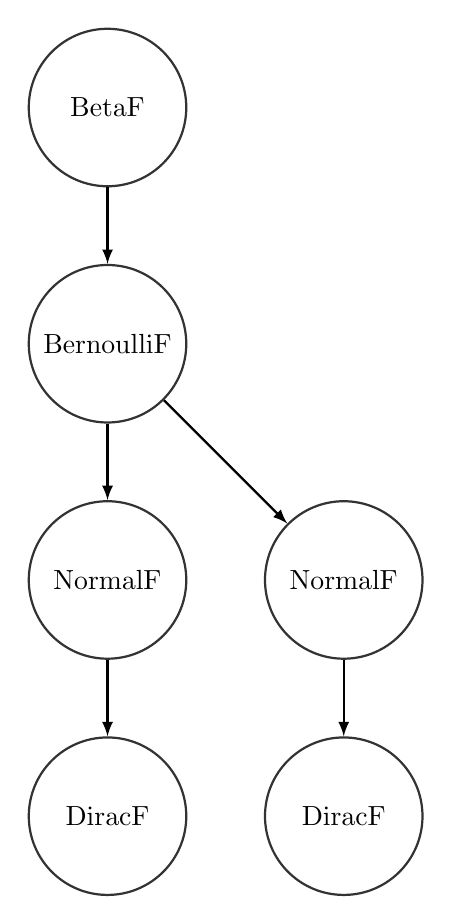
\begin{tikzpicture}

  \tikzstyle{random}=[circle, minimum size = 20mm, thick, draw = black!80, node distance = 30mm]
  \tikzstyle{connect}=[-latex, thick]

  \node[random] (beta) { \textrm{BetaF} };
  \node[random] (bernoulli) [below of = beta] { \textrm{BernoulliF} };
  \node[random] (gauss0) [below of = bernoulli] { \textrm{NormalF} };
  \node[random] (gauss1) [below of = bernoulli, right of = bernoulli] { \textrm{NormalF} };
  \node[random] (dirac0) [below of = gauss0] { \textrm{DiracF} };
  \node[random] (dirac1) [below of = gauss1] { \textrm{DiracF} };

  \path (beta) edge [connect] (bernoulli)
        (bernoulli) edge [connect] (gauss0)
        (bernoulli) edge [connect] (gauss1)
        (gauss0) edge [connect] (dirac0)
        (gauss1) edge [connect] (dirac1);

\end{tikzpicture}

\end{document}
